\chapter{Experiments and Results}
\label{chapter:ref}


\section{Dataset}
This research utilizes a welding defect dataset generously provided by an electronics manufacturing company, encompassing a vast collection of 1,364,400 images. Each image is intricately associated with a distinct defect category and the corresponding component name. The intricate nature of component welding processes introduces a variety of potential defects, thereby prompting the categorization into six defect types: Good (indicating normalcy), Missing, Shift, Stand, Broken, and Short, as shown in Figure 1.1.

It is important to note that the "Good" category contains a substantial number of component images, creating a noticeable imbalance compared to the relatively limited samples found in other defect categories-particularly within the realm of new components. This imbalance, notably in the new component subset, is a pivotal challenge in our dataset.

To mitigate this challenge, an over-sampling strategy has been employed on the original dataset. Given the scarcity of defect samples, the data's inherent imbalance is addressed by repeatedly sampling from the underrepresented class. This method involves the random duplication of instances, effectively augmenting the less abundant class to achieve a more equitable distribution of data between the two classes.

Additionally, the dataset was meticulously reorganized. Despite variations in nomenclature, certain components exhibit only subtle visual disparities due to the distinctive resistance characteristics of each component. To  prevent potential overfitting during the training phase, visually similar components were carefully grouped into the same category or cluster, forming cohesive and homogenous groups. For a more comprehensive understanding of this reorganization process, please refer to Section 3.1.

We generated a simplified yet representative dataset using OpenCV for training purposes. Distinguishing features within this dataset include variations in color intensity and changes in shape, which are considered unique attributes for different groups. Furthermore, defect types across different groups are characterized by the absence of corners and rotations, ranging from angles greater than 1 degree to less than 45 degrees. Each combination comprises 500 images, resulting in a total of 3 * 5 * 500 images, as illustrated in Figure 4.1.
\begin{figure}[H]
    \centering
    \includegraphics[width=1\linewidth]{Toy Dataset.png}
    \caption{Toy Dataset}
    \label{fig:enter-label}
\end{figure}

\section{Experimental Setup}
\label{sec:quote}
To refine our model, we utilized the Stable-diffusion-2-base pre-trained model on the LAION-5B dataset as a foundational framework, implementing PyTorch with default hyperparameters. The training epochs were set to 100, and the initial learning rate was configured as 5e-5. For optimization, we employed the CosineAnnealingLR, with training commencing after a warm-up scheduler for epochs/10.

Given the diverse sizes of components, all input images were resized uniformly to 64x64 color images. This standardized approach accommodated the inherent variability in component dimensions.

To augment our model's training set, random horizontal flip and random vertical flip techniques were employed, providing additional diversity for robust training. Notably, these augmentation strategies enhanced the model's ability to generalize across various component orientations.

In contrast, the validation and test sets were maintained in their original form without applying any image augmentation. This ensured a thorough evaluation of the model's performance on previously unseen data, thereby reflecting real-world scenarios.

All experiments were conducted using two high-performance NVIDIA Tesla V100 GPU, to optimize computational efficiency. 
\newpage
\section{Experiment Results}
The Compositional Conditional Diffusion Model (CCDM) provides a flexible and computationally tractable approach for synthesizing images across various modalities. We provide detailed information on the architecture, implementation, training, and evaluation of all the results presented in this section.Additionally, an overview of the hyperparameters of all trained CCDM is provided in this section.

\subsection{Toy Dataset}
Initially, we started by removing the instances from the Toy Dataset (as shown in Figure 4.1) corresponding to the "Broke Group1" and "Shift Group1." This exclusion ensures that these groups do not contribute to the training add a space in between the period and subsequently, we fed these modified datasets into the cMLIP model for training, striving to develop a pre-trained class-image model for utilization as an embedder in the conditional diffusion model.Tab 4.1 illustrates the hyperparameters employed in training the cMLIP model.
\begin{table}[H]
    \centering
    \renewcommand{\arraystretch}{1} % 調整行距
    \begin{tabular}[h]{lc} \hline 
        \multicolumn{2}{c}{cMLIP} \\ \hline
        Epoch & 10\\ 
        Batch size &  16\\ 
        Learning rate & 1e-4\\ 
        Dropout & 0.15\\
        Weight Decay & 1e-4\\
        Class embedding dimension & 512 \\
        Projection dimension & 256 \\ \hline 
    \end{tabular}
    \caption{The parameter settings of cMLIP in Toy Dataset}
    \label{tab:experimental_config}
\end{table}
After training, we compute the similarity between cMLIP image features and class features, followed by applying softmax. As shown in Tab 4.2, the images labeled as 'Broke Group1' and 'Shift Group1,' which are not present in the dataset, exhibit remarkably high probabilities in terms of accurate predictions.
\begin{table}[H]
    \centering
    \renewcommand{\arraystretch}{1} % 調整行距
    \begin{tabular}[h]{lcc} \hline 
        \multicolumn{3}{c}{cMLIP result} \\ 
        Group name& Top1(\%) & Top5(\%)\\ \hline
        Good Group1 & 100 & 100\\ 
        Good Group2 & 100 & 100\\ 
        Good Group3 & 100 & 100\\ 
        Good Group4 & 100 & 100\\ 
        Good Group5 & 100 & 100\\ 
        Broke Group1 (unseen) & 97 & 100\\ 
        Broke Group2 & 100 & 100\\ 
        Broke Group3 & 100 & 100\\ 
        Broke Group4 & 100 & 100\\ 
        Broke Group5 & 100 & 100\\ 
        Shift Group1 (unseen) & 76 & 100\\ 
        Shift Group2 & 100 & 100\\ 
        Shift Group3 & 100 & 100\\ 
        Shift Group4 & 100 & 100\\ 
        Shift Group5 & 100 & 100\\ \hline 
    \end{tabular}
    \caption{The outcomes of cMLIP in the Toy Dataset }
    \label{tab:experimental_config}
\end{table}
\begin{table}[H]
    \centering
    \renewcommand{\arraystretch}{1} % 調整行距
    \begin{tabular}[h]{lc} \hline 
        \multicolumn{2}{c}{Compositional Conditional Diffusion Model} \\ \hline
        Epoch & 100\\ 
        Batch size &  64\\ 
        Learning rate & 5e-5\\ 
        Optimizer & AdamW\\ 
        Diffusion steps & 1000\\ 
        Noise Schedule & linear \\ 
        Channel & 128 \\
        Depth & 2 \\ 
        Channel Multiplier & [1, 2, 2, 2]\\ 
        Head Channels & 4\\ 
        Dropout & 0.15\\
        Weight Decay & 1e-4\\
        Embedding Dimension & 512 \\ \hline 
    \end{tabular}
    \caption{The parameter settings of  CCDM in Toy Dataset}
    \label{tab:experimental_config}
\end{table}
In Figure 4.2, we can observe that both the U-Net 1 and U-Net 2 methods exhibit commendable performance in generating unseen images on the toy dataset. Through validation on this toy dataset, we establish the feasibility of these two approaches.
\begin{figure}[H]
    \centering
    \includegraphics[width=1\linewidth]{Toy PCB result (2).png}
    \caption{On the Toy dataset, the results generated by CCDM are presented using (a) the U-Net 1 method with learnable condition embedding, (b) the U-Net 1 method with fixed condition embedding(random), (c) the U-Net 2 method with fixed condition embedding (cMLIP), and (d) the U-Net 2 (AdaGN) method with fixed condition embedding (cMLIP).}
    \label{fig:enter-label}
\end{figure}
Upon careful examination of the outcomes, it is evident that using the U-Net 1 method with learnable condition embedding demonstrates superior performance in generating unseen images on the Toy dataset.

\subsection{PCB Dataset}
As depicted in Figure 1.1, however, we observed distinct patterns for the Broke samples in each Group. We specifically focused on the Broke pattern associated with missing corners. Therefore, we selected several Groups, namely Group1, Group4, Group5, and Group7, where the Broke patterns aligned with our criteria. The subsequent presentation aims to showcase the results obtained on the PCB dataset. Identical hyperparameters as the toy dataset were utilized during the training of cMLIP. Let us now delve into the details presented in Table 4.4.
\begin{table}[H]
    \centering
    \renewcommand{\arraystretch}{1} % 調整行距
    \begin{tabular}[h]{lc} \hline 
        \multicolumn{2}{c}{cMLIP} \\ \hline
        Epoch & 10\\ 
        Batch size &  16\\ 
        Learning rate & 1e-4\\ 
        Dropout & 0.15\\
        Weight Decay & 1e-4\\
        Class embedding dimension & 512 \\
        Projection dimension & 256 \\ \hline 
    \end{tabular}
    \caption{The parameter settings of cMLIP in PCB Dataset }
    \label{tab:experimental_config}
\end{table}
Due to the absence of Broke Group3 in the PCB Dataset, the calculation of its cosine similarity in cMLIP is not feasible. Nevertheless, it is evident that cMLIP demonstrates impressive performance on other observed data points.
\begin{table}[H]
    \centering
    \renewcommand{\arraystretch}{1} % 調整行距
    \begin{tabular}{lcc}
        \hline 
        \multicolumn{3}{c}{cMLIP result} \\ 
        Group name & Top1(\%) & Top5(\%)\\ \hline
        Good Group1 & 100 & 100\\ 
        Good Group3 & 97 & 100\\ 
        Good Group4 & 100 & 100\\ 
        Good Group5 & 100 & 100\\ 
        Good Group7 & 100 & 100\\ 
        Broke Group1 & 96 & 100\\ 
        Broke Group3 (unseen) &  & \\ 
        Broke Group4 & 100 & 100\\ 
        Broke Group5 & 100 & 100\\ 
        Broke Group7 & 100 & 100\\ 
        Shift Group1 & 100 & 100\\ 
        Shift Group3 & 100 & 100\\ 
        Shift Group4 & 100 & 100\\ 
        Shift Group5 & 97 & 100\\
        Shift Group7 & 99 & 100\\ \hline 
    \end{tabular}
    \caption{The outcomes of cMLIP in the PCB Dataset }
    \label{tab:experimental_config}
\end{table}
\begin{table}[H]
    \centering
    \renewcommand{\arraystretch}{1} % 調整行距
    \begin{tabular}{lc}
        \hline 
        \multicolumn{2}{c}{Compositional diffusion model} \\ \hline
        Epoch & 100\\ 
        Batch size & 64\\ 
        Learning rate & 5e-5\\ 
        Optimizer & AdamW\\ 
        Diffusion steps & 1000\\ 
        Noise Schedule & linear \\ 
        Channel & 128 \\
        Depth & 2 \\ 
        Channel Multiplier & [1, 2, 2, 2]\\ 
        Head Channels & 4\\ 
        Dropout & 0.15\\
        Weight Decay & 1e-4\\
        Embedding Dimension & 512 \\ \hline 
    \end{tabular}
    \caption{The parameter settings of CCDM in PCB Dataset }
    \label{tab:experimental_config}
\end{table}

In Figure 4.3, we can observe that both the U-Net 1 and U-Net 2 methods exhibit commend-
able performance in generating unseen images on the PCB dataset.
\begin{figure}[H]
    \centering
    \includegraphics[width=1\linewidth]{PCB dataset Result.png}
    \caption{On the PCB dataset, the results generated by CCDM are presented using (a) the U-Net 1 method with learnable condition embedding, (b) the U-Net 1 method with fixed condition embedding(random), (c) the U-Net 2 method with fixed condition embedding (cMLIP), and (d) the U-Net 2 (AdaGN) method with fixed condition embedding (cMLIP)}
    \label{fig:enter-label}
\end{figure}

During the PCB dataset image sampling process, we observed that U-Net 2 and U-Net 1 with fix embedding are failed to generate images accurately, whereas U-Net 1 with learnable condition embedding could generate images correctly, albeit with a high error rate. Some generated images exhibited discrepancies with the specified compositional conditions. In Figure 4.4, we sampled 50 images of unseen images (broke group 3), revealing a relatively low accuracy. Subsequently, we employed a simple binary classifier to train on the original PCB dataset, enabling the classifier to distinguish between broke and unbroke instances. This approach aimed to refine the selection of accurate images by leveraging the binary classifier's ability to discern the presence of defects.

\begin{figure}[H]
    \centering
    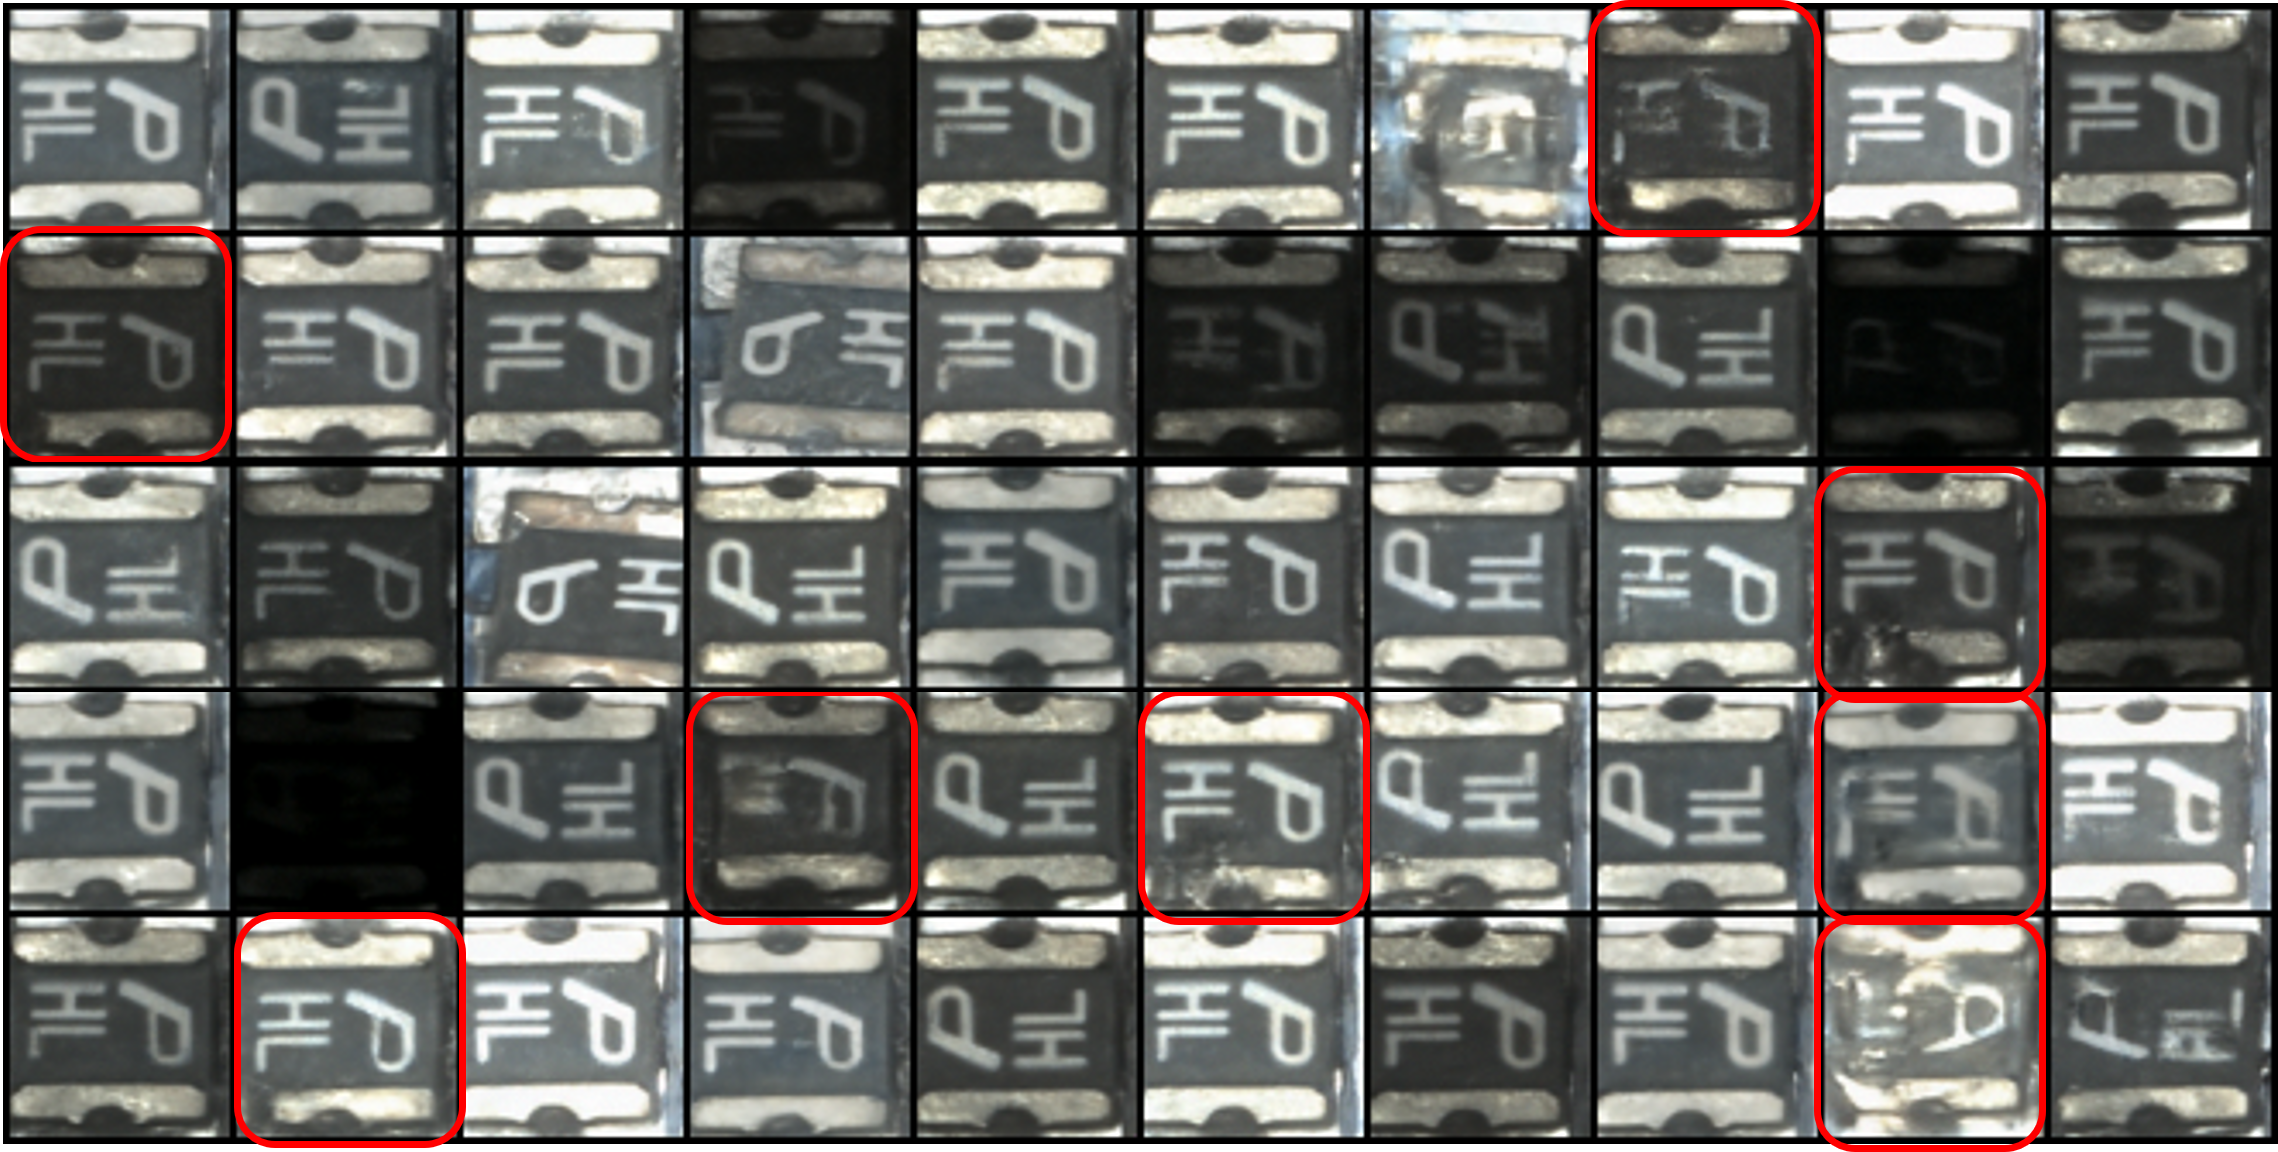
\includegraphics[width=0.75\linewidth]{PCB unseen image sample.png}
    \caption{The highlighted portion in the red box represents the results selected by the binary classifier, further refined through manual curation.}
    \label{fig:enter-label}
\end{figure}

Due to the lack of actual Broke Group3 samples, we conducted an experiment using ResNet152 as the backbone for our classifier, training it on the PCB Dataset categorized into Good, Broken, and Shifted. Initially, without incorporating Broke Group1, the classifier's accuracy in correctly identifying real instances of Broke Group1 was approximately 22\%. Subsequently, we included Broke Group1 instances generated by CCDM into the classifier's training regimen. This integration led to a significant improvement, enabling the classifier to achieve around 75\% accuracy in identifying authentic Broke Group1 instances. 

Finally, I added some raw images from Broke Group1 into the training data so that the dataset would not be entirely without Broke Group1, mimicking the typical structure of real data. Initially, the result was 97\%. After incorporating photos generated by our CCDM as an augmented dataset, the accuracy improved to 98\%. 

This result demonstrates our success in generating new component defect images, which serves as an expansion of the dataset for defect detection applications.Figure 4.5 is generated by selecting an image produced by U-Net 1 with learnable condition embedding, specifically from broke Group3.

\begin{figure}[H]
    \centering
    \includegraphics[width=0.75\linewidth]{Generate image.png}
    \caption{The image generated after selecting an image using U-Net 1 with learnable condition embedding.}
    \label{fig:enter-label}
\end{figure}